\chapter{Frame del dataset de demostraciones}
\label{apx:frame}

\lettrine{E}{n} este apéndice se muestra un ejemplo real de un \emph{frame} del
conjunto de demostraciones generado por el agente simbólico
(Capítulo~\ref{chap:iter1}). Cada \emph{frame} es un par \textit{OBSERVACIÓN-ACCIÓN}: la
imagen del visor en primera persona (Figura~\ref{fig:apx-frame}, página~\pageref{apx:frame}) junto con el
registro JSON de su estado, su acción y los metadatos de percepción
(Listado~\ref{lst:frame}, página~\pageref{lst:frame}).

\begin{figure}[hp!]
  \centering
  \resizebox{\textwidth}{!}{
  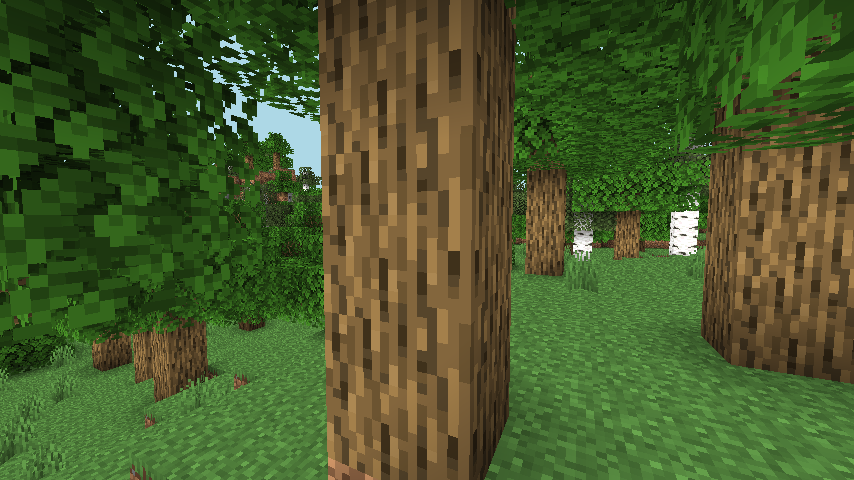
\includegraphics[width=0.8\textwidth]{imaxes/anexos/imagen_visor.png}
  }
  \caption[Imagen del visor en primera persona]{Imagen del visor en primera persona asociada al \emph{frame} del
  Listado~\ref{lst:frame} (página~\pageref{lst:frame}): el agente apunta a un tronco situado a $2{,}7$ bloques y
  ejecuta la acción \texttt{attack}.}
  \label{fig:apx-frame}
\end{figure}

\clearpage
\begin{lstlisting}[caption={Registro JSON de un \emph{frame} (par \textit{OBSERVACIÓN-ACCIÓN}) del dataset de demostraciones.},label={lst:frame}]
{
  "image": "data/recordings/Rec_100_ablgs0_screenshots/frame_00003.png",
  "state": {
    "x": 11.499,
    "y": 123,
    "z": 6.581,
    "yaw": -3.1416,
    "pitch": -0.343
  },
  "action": "attack",
  "camera_delta": {
    "dyaw": 0,
    "dpitch": 0
  },
  "session_id": "Rec_100_ablgs0",
  "tree_visible": true,
  "tree_distance": 2.7
}
\end{lstlisting}

En este \emph{frame}, el agente tiene un tronco visible a $2{,}7$ bloques
(\texttt{tree\_visible}~=~true) y ejecuta la acción \texttt{attack} sin
desplazamiento de cámara (\texttt{camera\_delta} nulo), correspondiente al instante
en que tala el árbol que tiene enfrente. 